\renewcommand*{\arraystretch}{1.1}

\subsection*{BI / read / 19}
\label{section:bi-read-19}

\noindent\begin{tabularx}{\queryCardWidth}{|>{\queryPropertyCell}p{\queryPropertyCellWidth}|X|}
	\hline
	query & BI / read / 19 \\ \hline
%
	title & Stranger's interaction
 \\ \hline
%
	pattern & \hfill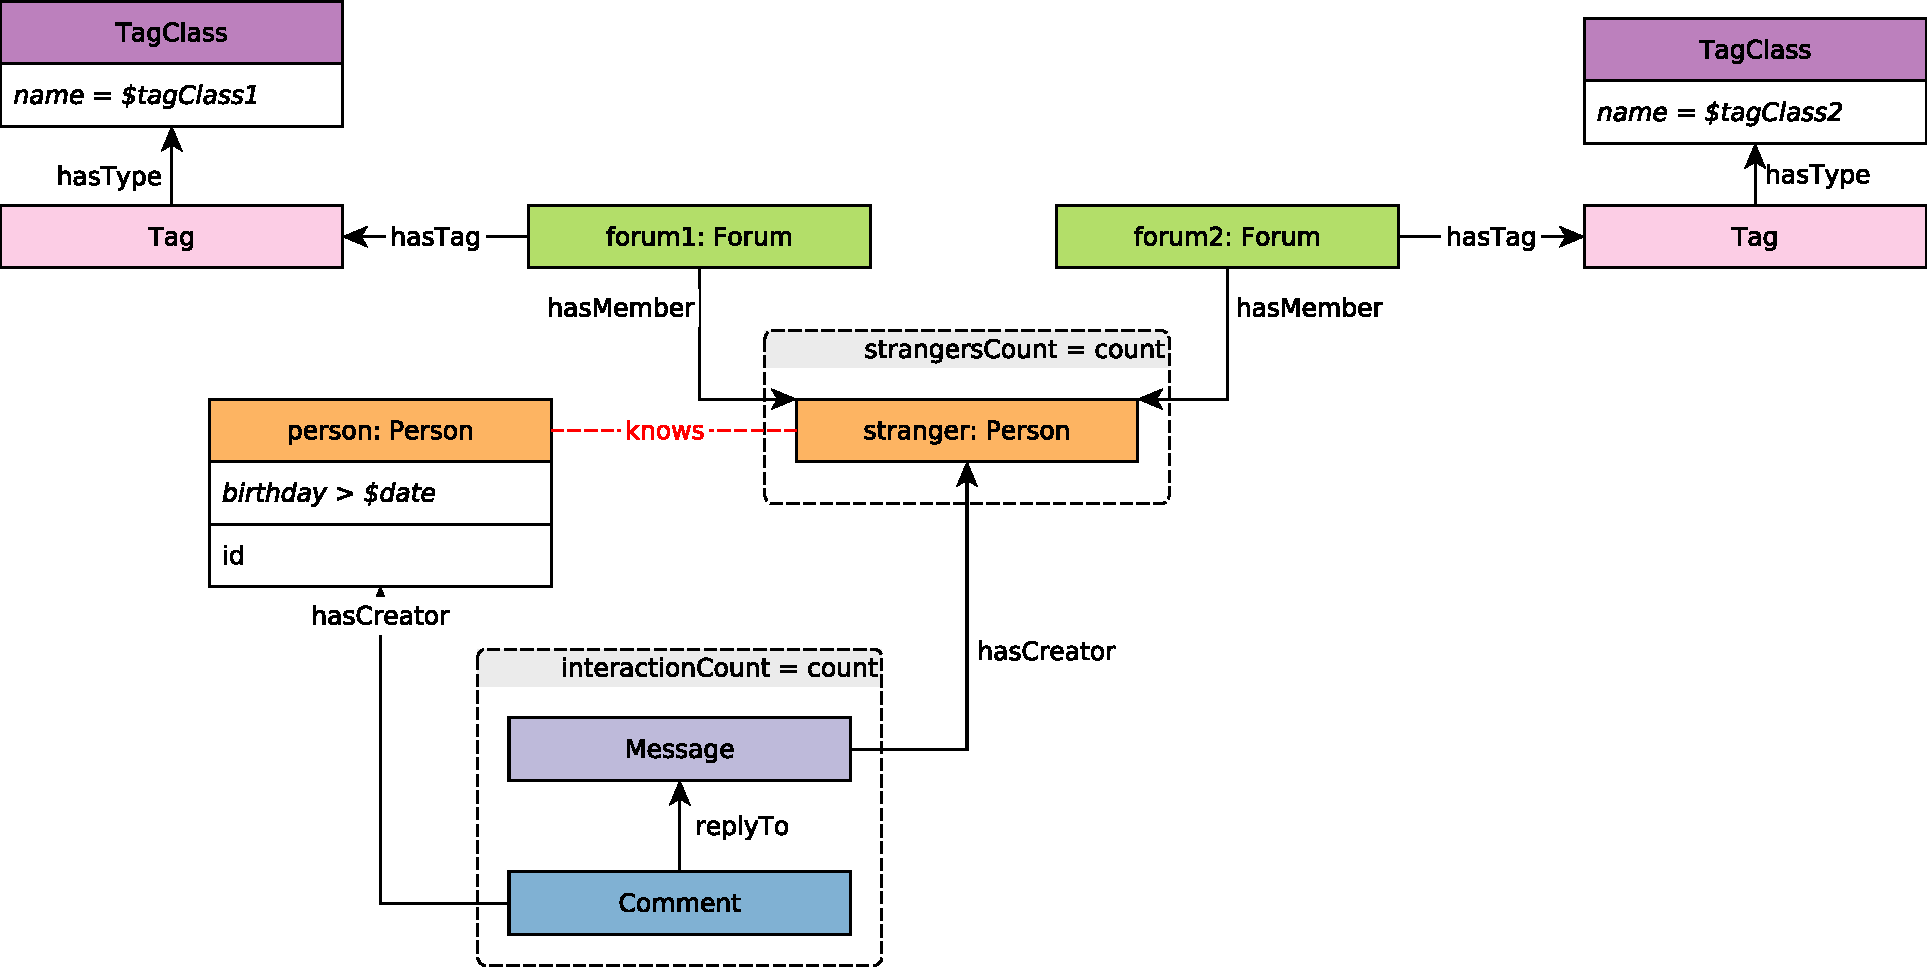
\includegraphics[scale=\patternscale,margin=0cm .2cm]{patterns/bi-read-19}\hfill\vadjust{} \\ \hline
%
	desc. & For all the Persons born after a certain date, find all the strangers
they interacted with, where strangers are Persons that do not Know each
other. There is no restriction on the date that strangers were born.

Consider only strangers that are members of Forums tagged with tagClass1
(direct children not transitive) AND members of Forums tagged with
tagClass2 (direct children not transitive). It does not matter if these
Tags are attached to the same Forum, or different Forums.

Interaction is defined as follows: if Person \emph{A} replies to a
Message (Post or Comment) by another Person \emph{B}, there is a
``interacted with'' relationship from \emph{A} to \emph{B}. Note that
the ``interacted with'' relationship is directed.

For each Person, count the number of strangers they interacted with and
total number of times they interacted with them.
 \\ \hline
%
	
		params &
		\innerCardVSpace{\begin{tabularx}{\attributeCardWidth}{|>{\paramNumberCell}c|>{\varNameCell}M|>{\typeCell}m{\typeWidth}|Y|} \hline
		$\mathsf{1}$ & date
 & Date
 &  \\ \hline
		$\mathsf{2}$ & tagClass1
 & 32-bit Integer
 &  \\ \hline
		$\mathsf{3}$ & tagClass2
 & 32-bit Integer
 &  \\ \hline
		\end{tabularx}}\innerCardVSpace \\ \hline
	
%
	
		result &
		\innerCardVSpace{\begin{tabularx}{\attributeCardWidth}{|>{\resultNumberCell}c|>{\varNameCell}M|>{\typeCell}m{\typeWidth}|>{\resultOriginCell}c|Y|} \hline
		$\mathsf{1}$ & person.id
 & 64-bit Integer
 & R &
				 \\ \hline
		$\mathsf{2}$ & strangersCount
 & 32-bit Integer
 & R &
				 \\ \hline
		$\mathsf{3}$ & interactionCount
 & 32-bit Integer
 & R &
				 \\ \hline
		\end{tabularx}}\innerCardVSpace \\ \hline
	
%
	
		sort		&
		\innerCardVSpace{\begin{tabular}{|>{\sortNumberCell}c|>{\varNameCell}l|>{\directionCell}c|} \hline
		$\mathsf{1}$ & interactionCount
 & $\desc
$ \\ \hline
		$\mathsf{2}$ & person.id
 & $\asc
$ \\ \hline
		\end{tabular}}\innerCardVSpace \\ \hline
	%
	limit & 100 \\ \hline
	%
	CPs &
	\multicolumn{1}{>{\raggedright}l|}{
		\chokePoint{1.1}, 
		\chokePoint{1.4}, 
		\chokePoint{2.1}, 
		\chokePoint{2.3}, 
		\chokePoint{2.4}, 
		\chokePoint{3.3}, 
		\chokePoint{5.1}, 
		\chokePoint{7.3}, 
		\chokePoint{7.4}
		} \\ \hline
	%
	%
\end{tabularx}
\queryCardVSpace